\FloatBarrier
\section{Large-Drive Spectroscopy}
\label{sec:high-amplitude-regime}

\subsection{Broad and Narrow Frequency Scans}
\label{subsec:broad-and-narrow-scans}

High-resolution spectroscopy at large drive amplitudes is characterized on two
frequency scales.  A broad scan first locates the qubit transition and reveals
the surrounding baseline, nearby spectral features, and any strong-drive
distortions.  A narrow scan centered on the transition then samples the sharp
echo--root--Lorentzian depletion feature densely enough to determine its center
and linewidth.  Presenting the broad and narrow scans together distinguishes a
genuinely narrow resonance from a local feature embedded in a wider distorted
response and demonstrates that the high resolution persists within the full
spectral landscape.

\subsection{Extended-Amplitude Regime and Strong-Drive Distortions}
\label{subsec:extended-amplitude-regime}

At drive amplitudes above approximately $50~\mathrm{MHz}$, the Rabi frequency
is no longer small compared with the transmon anharmonicity and the measured
response begins to depart from an effective two-level description.  Possible
mechanisms include coupling
to higher transmon levels, drive-induced level shifts, leakage, and
multiphoton processes~\cite{PhysRevA.76.042319,motzoi_drag_2009,tuorila_stark_2010}.  The two-level calculation in
Sec.~\ref{sec:numerical-model} cannot distinguish among these mechanisms, so
the additional structure is reported here as a strong-drive distortion rather
than assigned to a specific transition.  Quantitative attribution would
require a converged multilevel model and an independent calibration of the
delivered drive amplitude.

\subsection{Cutoff Dependence from 50 to 80 MHz}
\label{subsec:high-amplitude-cutoff-comparison}

To separate large-drive behavior from changes in pulse duration or sampling,
we compare three q1 echo--root--Lorentzian scans acquired with the same
$10~\mu\mathrm{s}$ duration, detuning grid, amplitude grid, active-reset
protocol, and 40 repetitions per point.  Only the dimensionless cutoff-control
setting is changed, from $c=0.001$ to 0.005 and 0.010.  Using the same-day q1
$\pi$-pulse calibration retained with the data, the displayed portion of each
scan is selected from raw peak Rabi frequencies of $50.28$ to
$76.97~\mathrm{MHz}$.  The centers of the displayed block averages span
$50.67$ to $76.19~\mathrm{MHz}$.  This
restricted view exposes the high-amplitude response directly instead of
allowing the much larger low-amplitude region to dominate the color scale.
To reduce binomial sampling noise without imposing a fit or interpolated
surface, each displayed cell is a non-overlapping average of three adjacent
detuning points and three adjacent amplitude points.  Since every raw point
contains 40 repetitions, a displayed cell averages 360 binary outcomes.

Figure~\ref{fig:high-amplitude-cutoff-comparison} shows a pronounced
reorganization of the large-drive response with cutoff.  At $c=0.001$ the map
is dominated by a step-like change across zero detuning, whereas the
$c=0.005$ and 0.010 scans develop curved, amplitude-dependent fringes that
cross the central-frequency region.  Thus these measurements do not support
extrapolating the low-amplitude narrow-feature behavior unchanged into the
$50$--$80~\mathrm{MHz}$ regime.  Instead, they identify a cutoff-sensitive
strong-drive regime in which a single-linewidth description is insufficient.
Because all panels use one color scale, the differences are not artifacts of
independent normalization.

\begin{figure}[t]
    \centering
    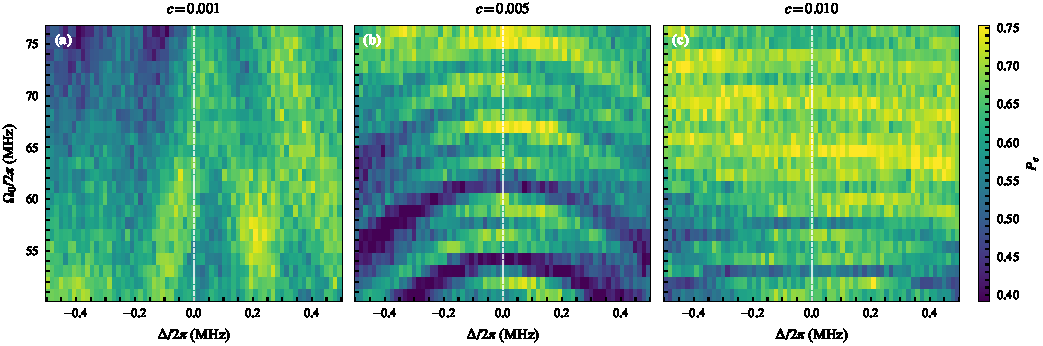
\includegraphics[width=1\linewidth]{../figures/paper/07_high_amplitude_cutoff_comparison.pdf}
    \caption{Measured high-amplitude echo--root--Lorentzian spectroscopy on
    q1 for dimensionless cutoff-control settings (a) $c=0.001$,
    (b) $c=0.005$, and (c) $c=0.010$.  Each panel shows the same
    $50.28$--$76.97~\mathrm{MHz}$ raw peak-Rabi-frequency interval from a
    $10~\mu\mathrm{s}$ scan with 40 repetitions per point.  The dashed line
    marks zero detuning, and all panels share the color scale.  Displayed cells
    are non-overlapping $3\times3$ block averages of the measured grid; no
    interpolation or fitted surface is shown.  The progression
    from a step-like response in (a) to curved interference fringes in (b) and
    (c) demonstrates that the large-drive structure is cutoff sensitive.}
    \label{fig:high-amplitude-cutoff-comparison}
\end{figure}
\FloatBarrier

\begin{figure}[t]
    \centering
    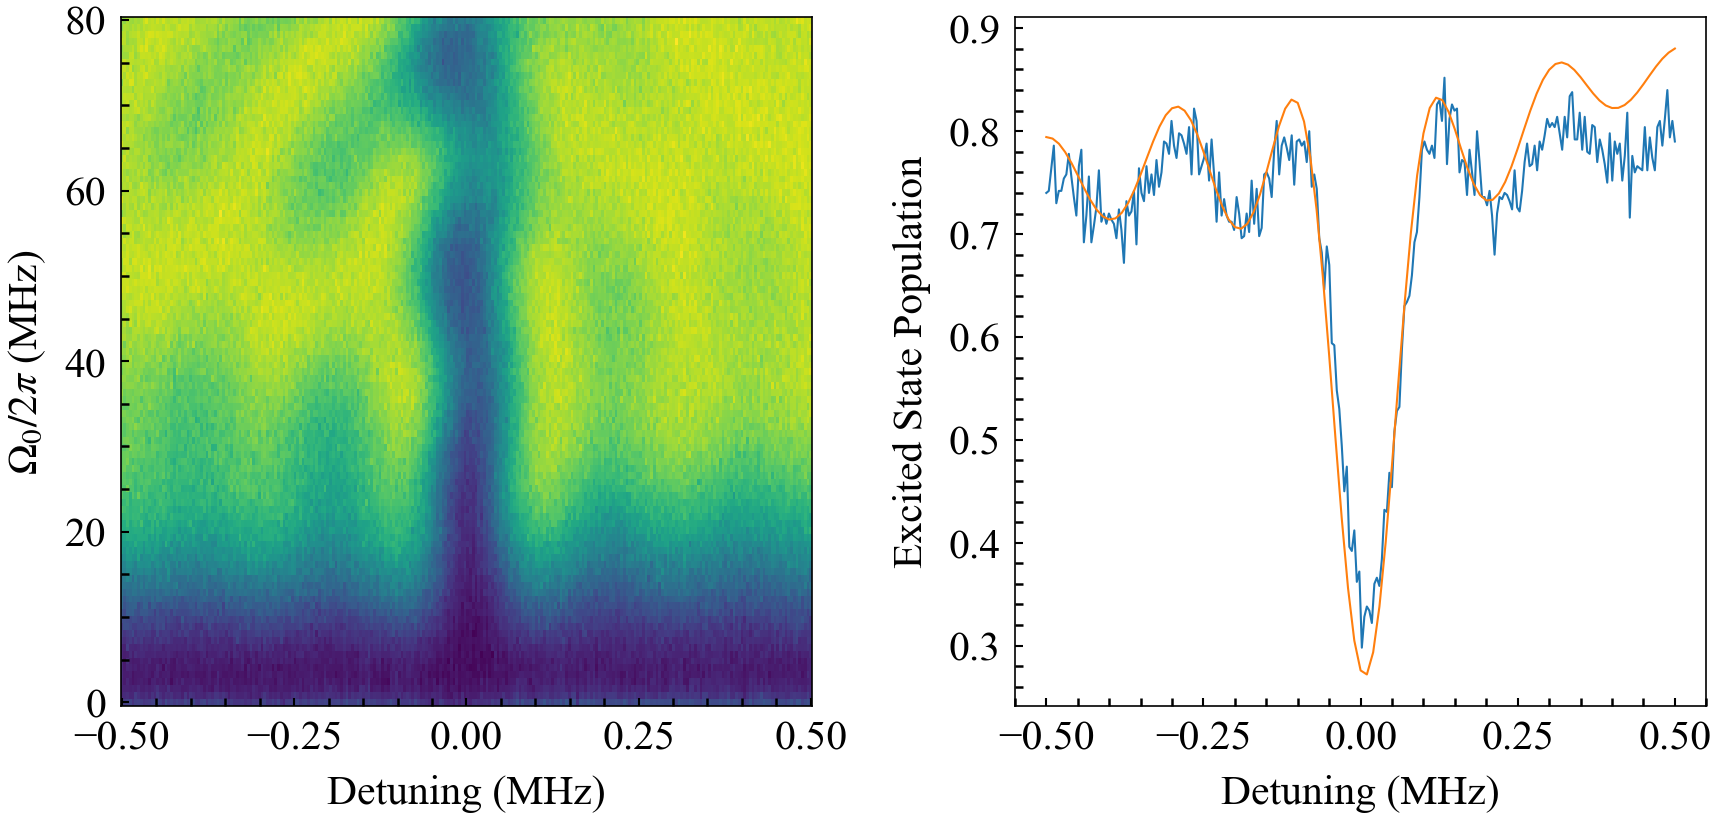
\includegraphics[width=1\linewidth]{figures/comparison.png}
    \caption{Two-dimensional spectroscopy map obtained with a
    $10~\mu\mathrm{s}$ echo--root--Lorentzian pulse at extended drive
    amplitudes (up to $80~\mathrm{MHz}$).  The left panel shows the full
    detuning--amplitude map, while the right panel presents a line cut at fixed
    drive strength (blue) together with a smooth fit (orange).  The observed
    distortions mark the breakdown of the ideal effective two-level response
    as the drive approaches the multilevel regime.}
    \label{fig:high-amplitude-comparison}
\end{figure}
\FloatBarrier
